\chapter{Interpolation}

\underline{Beispiel}: Gegeben sind Temperaturen $f_0, f_1, f_2, \hdots$ gemessen zu bestimmten Zeitpunkten $x_0,x_1,x_2\hdots$

\bigskip

\underline{Frage}: Wie ist die Temperatur zu einem Zeitpunkt $\hat x$ mit $\hat x\neq x_i$?

\begin{center}
    \begin{tikzpicture}
    \draw[->] (-1,0) -- (7,0);
    \draw[->] (0,-1) -- (0,4);
    \draw (-0.5,3.5) node {$f$};
    \foreach \i in {0,1,2,3,4,5}
        {
            \draw (\i + 1,0) node[below] {$x_{\i}$};
            \draw (\i + 1, 0.05) -- (\i+1,-0.05);
        }
     \draw plot[smooth] coordinates { (1,2) (2,3) ( 3,3) (4,2) (5,2) (6,1) };
     \foreach \x/\y in { 1/2, 2/3, 3/3, 4/2, 5/2, 6/1}
     {
        \draw (\x-0.1,\y+0.1) -- (\x+0.1,\y-0.1);
        \draw (\x-0.1,\y-0.1) -- (\x+0.1,\y+0.1);
     }
    \end{tikzpicture}
\end{center}

\underline{Idee:} \begin{itemize}
                   \item  Finde eine \glqq sinnvolle\grqq~Funktion $f: x\mapsto f(x)$ mit $f(x_i)=f_i\quad \forall i$
                    \item Die gesuchte Temperatur ist $f(\hat x)$\\
                    $\rightarrow$ \glqq intelligent geraten\grqq
                  \end{itemize}

\bigskip

\begin{definition}[Interpolationsproblem]
 Gegeben:
 \begin{itemize}
  \item $n+1$ Stützstellen $x_0,\hdots,x_n\in\R$, paarweise verschieden,
  \item $n+1$ Stützwerte $f_0,\hdots,f_n\in\R$.
 \end{itemize}
Finde eine \glqq sinnvolle\grqq~Funktion $f:\R\to\R$ mit $f(x_i)=f_i\ \forall i=0,\hdots,n$.
\end{definition}


Was heißt \glqq sinnvoll\grqq ?
\begin{itemize}
 \item Eindeutig bestimmt in einer fixen Funktionsklasse
 \item Möglichst billig auszurechnen
 \item Kleiner Fehler
 \item \glqq sinnvoll\grqq~ist kein mathematischer Begriff -- es kann Wissen aus der Anwendung dazukommen.
\end{itemize}

\section{Polynominterpolation}

\begin{itemize}
 \item Versuche, $f$ als Polynom zu konstruieren.
 \item Guter Kompromiss zwischen Flexibilität und einfacher Handhabung
\end{itemize}

Polynom $n$-ten Grades:
\begin{equation*}
    p(x) \coloneqq a_n x^n + a_{n-1}x^{n-1} + \hdots + a_1 x + a_0\quad \forall x\in\R,\ a_n\neq 0
\end{equation*}

Sei $\Pi_n$ die Menge aller Polynome vom Grad höchstens $n$.

\bigskip

Vielversprechender Ansatz:
\begin{itemize}
  \item $n+1$ Bedingungen $f(x_i)=f_i,\quad i=0,\hdots,n$
  \item $n+1$ freie Parameter $a_0,\hdots,a_n$
\end{itemize}

Kann man die Parameter so wählen, dass die Interpolationsbedingung erfüllt ist?\\

\subsection{Lagrange-Interpolation}

Konstruktion: Definiere $L_j : \R\to\R$ durch
\begin{equation*}
 L_j(x)\coloneqq \prod_{\stackrel{i=0}{i\neq j}}^n \frac{x-x_i}{x_j-x_i} = \frac{(x-x_0)(x-x_1) \cdots (x-x_{j-1})(x-x_{j+1}) \cdots (x-x_n)}{(x_j-x_0)(x_j-x_1) \cdots (x_j-x_{j-1})(x_j-x_{j+1}) \cdots (x_j-x_n)}
\end{equation*}
$\rightarrow$ Polynom vom Grad $n$\\ (der Nenner ist eine feste Zahl $\neq 0$, die nur von den Stützstellen abhängt)

\medskip

Werte an den Stützstellen:
\begin{equation*}
 L_j(x_k)
 =
 \delta_{jk}
 \colonequals
 \begin{cases}
  0 & \text{falls $j\neq k$} \\
  1 & \text{falls $j=k$}
 \end{cases}
\end{equation*}
(\qq{Lagrange-Eigenschaft})\\

\underline{Joseph-Louis Lagrange}
\begin{itemize}
 \item geb.~1736 in Turin als Guiseppe Lodovico Lagrangia
 \item gest.~1813 in Paris
 \item Mit 19 Lehrstuhl für Mathematik an der Königlichen Artillerieschule in Turin
 \item Ab 1766: Nachfolger von Leonard Euler (als Direktor) an der Preußischen Akademie der Wissenschaften in Berlin
 \item 1786 (Tod von Friedrich II) $\rightarrow$ Paris
 \item Napoleon machte ihn zum Grafen
 \item Im Pantheon begraben
 \item Auf dem Eiffelturm verewigt
\end{itemize}
Variationsrechnung: Lagrange-Multiplikatoren\\
Analysis: Lagrange-Restglied der Taylor-Formel

\bigskip

Definiere $p:\R\to\R$ durch
\begin{equation*}
 p(x) \coloneqq \sum_{j=0}^n f_j L_j(x)
\end{equation*}
(Lagrange-Form des Interpolationspolynoms)
\begin{itemize}
 \item Polynom $n$-ten Grades
 \item erfüllt die Interpolationsbedingung:
 \begin{equation*}
  p(x_i) = \sum_{j=0}^n f_jL_j(x_i) = \sum_{j=0}^n f_j \delta_{ij} = f_i
 \end{equation*}
\end{itemize}

Wir haben bewiesen:
\begin{satz}
 Zu $n+1$ beliebigen Datenpaaren $(x_0,f_0),\hdots,(x_n,f_n)$ mit paarweise verschiedenen Stützstellen existiert ein Polynom $p\in\Pi_n$, das die Interpolationsbedingung erfüllt.
\end{satz}

\begin{satz}
 Dieses Polynom ist eindeutig.
\end{satz}
\begin{proof}
 Seien $p,\tilde p\in\Pi_n$ beides Interpolationspolynome.
 \begin{itemize}
  \item Dann ist $p-\tilde p \in \Pi_n$.
  \item Für die Stützstellen $x_k,\ k=0,\hdots,n$ gilt
  \begin{equation*}
    (p-\tilde p)(x_k) = p(x_k) - \tilde p(x_k) = f_k - f_k = 0.
  \end{equation*}
  \item $p - \tilde p$ hat also mindestens $n+1$ Nullstellen.
 \end{itemize}
 $\Rightarrow$ Dann ist $p-\tilde p$ die Nullfunktion.
\end{proof}


\subsubsection{Aufwand der Lagrange-Interpolation}
\begin{itemize}
 \item Auswerten eines einzelnen $L_j$ an einer Stelle $x$:  $\mathcal{O}(n)$  Operationen
 \item Berechnen der Summe $\displaystyle p(x) = \sum_{j=0}^n f_jL_j(x) $: \quad $\mathcal{O}(n)$ Operationen
 \item Zusammen also $\mathcal{O}(n^2)$
 \item Auswertung an einem anderen Punkt: wieder $\mathcal{O}(n^2)$ Operationen.
\end{itemize}

\subsection{Newton-Form des Interpolationspolynoms}

\begin{definition}
 Die Newton-Form des Interpolationspolynoms $p$ ist
 \begin{equation*}
  p(x) = c_0 + c_1(x-x_0) + c_2(x-x_0)(x-x_1) + \hdots + c_n(x-x_0)(x-x_1)\cdots (x-x_{n-1})
 \end{equation*}
 mit passenden Koeffizienten $c_0,\hdots,c_n\in\R$.
\end{definition}

\subsubsection{Wie berechnet man die Koeffizienten?}

Induktiv:

\medskip

Induktions-Anfang: $f_0 = p(x_0) = c_0$

\medskip

Induktions-Schritt: Seien $c_0,\hdots,c_{j-1}$ bereits bekannt
\begin{align*}
    f_j &= p(x_j) \\
       &= c_0 + \sum_{k=1}^{j-1} c_k(x_j-x_0)\cdots (x_j-x_{k-1}) + c_j \underbrace{(x_j-x_0)\cdots (x_j-x_{j-1})}_{ \neq 0} + \underbrace{0+\hdots 0}_{n-j \text{ viele}} \\
\end{align*}
Also:

\begin{equation*}
 c_j = \frac{f_j - c_0 - \sum_{k=1}^{j-1} c_k(x_j-x_0)\cdots (x_j-x_{k-1})}{(x_j-x_0)\cdots (x_j-x_{j-1})}
\end{equation*}

Diese Prozedur entspricht gerade dem Lösen eines linearen Gleichungssystems mit unterer Dreicksmatrix:
\begin{equation*}
 \begin{pmatrix}
    1 & & & & \\
    1 & (x_1-x_0) & & & \\
    1 & (x_2-x_0) & (x_2-x_0)(x_2-x_1) & & \\
    \vdots & \vdots & \vdots & \ddots & \\
    1 & (x_n-x_0) & \cdots & \cdots & \prod_{i=0}^{n-1}(x_n-x_i)
 \end{pmatrix} \begin{pmatrix}
    c_0 \\ c_1 \\ \vdots \\ \vdots \\ c_n
 \end{pmatrix} =
 \begin{pmatrix}
    f_0 \\ f_1 \\ \vdots \\ \vdots \\ f_n
 \end{pmatrix}
\end{equation*}

Vorteil der Newton-Form: Neue Stützstellen können mit wenig Aufwand hinzugefügt werden.
Bei der Lagrange-Form muss stattdessen alles komplett neu ausgerechnet werden.

\subsubsection{Aufwand}

\begin{itemize}
 \item Die Matrix kann in $\mathcal{O}(n^2)$ (genauer: $\frac{1}{2} n^2$) Operationen aufgestellt werden.
 \item Ist die Matrix bekannt, so kann das System in $\mathcal{O}(n^2)$ Schritten gelöst werden.
 \item Man braucht also $\mathcal{O}(n^2)$ Operationen, um die Koeffizienten $c_0,\hdots,c_n$ zu bestimmen.
\end{itemize}
Angenommen, die Koeffizienten seien jetzt bekannt. Auswerten an festem $x$:
 \begin{equation*}
  p(x) = c_0 + c_1(x-x_0) + c_2(x-x_0)(x-x_1) + \hdots + c_n(x-x_0)(x-x_1)\cdots (x-x_{n-1})
 \end{equation*}
 Naiv: $\frac{n(n - 1)}{2}$ Multiplikationen

 \bigskip

 Schlauer: Ausklammern!
 \begin{equation*}
  p(x) = c_0 + (x-x_0) \Big( c_1 + (x-x_1)\big( c_2 + (x-x_2) \ldots \big)\Big)
 \end{equation*}
 Algorithmus zum Ausrechnen von $p_0=p(x)$:
 \begin{align*}
  p_n &= c_n \\
  p_{n-1} &= c_{n-1} + (x-x_{n-1})\, p_n \\
  p_{n-2} &= c_{n-2} + (x-x_{n-2})\, p_{n-1} \\
          & \;\; \vdots \\
  p_0 &= c_0 + (x-x_0)\, p_1
 \end{align*}
 $\Rightarrow$ $n-1$ Multiplikationen $\rightarrow$ Horner-Schema\\
 Nach William George Horner, 1786 (Bristol) - 1837 (Bath)
 \begin{itemize}
  \item Direktor einer Schule in Bath
 \end{itemize}


 % Datum: 14.10.2015 
 
 \subsection{Interpolationsfehler}
 
 Welchen \qq{Fehler} macht man bei der Interpolation?
 \begin{itemize}
  \item Unklar: was heißt \qq{Fehler}?
  \item Idee: Die gegebenen Werte sind Funktionswerte einer stetigen Funktion.
 \end{itemize}
 
 \begin{definition}[Interpolationsproblem II]
  Sei $f\in C[a,b]$ gegeben und
  \begin{equation*}
   a \leq x_0 < x_1 < \hdots < x_n \leq b
  \end{equation*}
  Stützstellen. Finde ein $p\in\Pi_n$ so dass $p(x_i)=f(x_i)\ \forall i=0,\hdots,n$.
 \end{definition}
 \begin{definition}
  Der Interpolationsfehler ist
  \begin{equation*}
   \norm{f-p}_\infty \colonequals \max_{x\in[a,b]} \abs{ f(x) - p(x)}.
  \end{equation*}
   \end{definition}
$\rightarrow$ Diesen Wert hätten wie gerne klein.

\medskip

Geht das? Im Prinzip ja.

\begin{satz}[Weierstraß]
 Sei $f\in C[a,b]$. Dann existiert eine Folge $p_0,p_1,p_2,\hdots$ mit $p_n\in\Pi_n$, so dass $\norm{f-p}_\infty \stackrel{n\to\infty}{\longrightarrow} 0$.
\end{satz}

\begin{proof}
Funktionalanalysis, 5.~Semester.
\end{proof}

Karl Weierstraß 1815--1897
\begin{itemize}
 \item Ab 1841 Gymnasiallehrer an verschiedenen Orten in Deutschland
 \item Ab 1856 $\rightarrow$ Professor in Berlin
 \item Solide Fundierung der Analysis (\qq{weierstraßsche Strenge})
 \item Konvergenzkriterien für Reihen
 \item gleichmäßige Konvergenz
 \item Satz von Bolzano--Weierstraß
\end{itemize}


Kann man solche Polynome durch Interpolation konstruieren?

\bigskip

\underline{Hoffnung:} Mehr Stützstellen $\rightarrow$ kleinerer Fehler
\begin{equation*}
 \lim \norm{ f-p }_\infty = 0 \qquad \text{für immer feinere Aufteilung von $[a,b]$}.
\end{equation*}

\fbox{
Beispiele: [Computer]\\
}

\bigskip

Beispielfunktion von Carl Runge (1856--1927):
\begin{equation*}
       f(x) = \frac{1}{1+25x^2}
\end{equation*}


Warum geht das schief?

\bigskip

\begin{itemize}
 \item [Grund I:] Uniform verteilte Stützstellen sind böse! (Den Grund sehen wir gleich)

 \item [Grund II:] Die Runge-Funktion ist zwar $C^\infty$, aber die Werte der Ableitungen wachsen für höhere Ableitungsordnung:
\begin{equation*}
    \max_{[a,b]} \left\vert \frac{d^k}{dx^k} \left(\frac{1}{1+25x^2} \right) \right\vert
    \quad  \stackrel{k\to\infty}{\longrightarrow} \quad
    \infty.
\end{equation*}
\end{itemize}

Können wir etwas beweisen?

\medskip

Definiere die Hilfsfunktion $w:\R\to\R$
\begin{equation*}
 w(x) \coloneqq (x-x_0)(x-x_1)\cdots (x-x_n).
\end{equation*}

\begin{satz}
\label{thm:interpolation:interpolation_error}
 Sei $f\in C^{n+1}[a,b]$ und $a \leq x_0 < x_1 < \hdots < x_n \leq b$. Sei $p_n\in\Pi_n$ das dazugehörige Interpolationspolynom. Dann existiert zu jedem $x\in[a,b]$ eine Zahl $\xi_x\in(a,b)$, so dass
 \begin{equation} \label{eq:interpolation1}
    f(x) - p_n(x) = \frac{f^{(n+1)} (\xi_x)}{(n+1)!} \, w(x).
 \end{equation}
 Insbesondere gilt also
 \begin{equation*}
    \norm{ f - p_n}_\infty \leq \frac{1}{(n+1)!}\, \norm{ f^{(n+1)}}_\infty \norm{w}_\infty.
 \end{equation*}
\end{satz}

\begin{proof}
  Fall 1: Sei $x=x_k$ eine Stützstelle.  Dann folgt
  \begin{equation*}
   f(x)=p_n(x),\quad w(x)=0,
  \end{equation*}
  und \eqref{eq:interpolation1} ist mit jedem $\xi_x\in (a,b)$ erfüllt.

  \bigskip

  Fall 2: Sei $x\neq x_k\ \forall k=0,\hdots,n$.
  \begin{itemize}
   \item  Definiere Hilfsfunktion $g:[a,b]\to\R$
  \begin{equation*}
    g(t) \coloneqq f(t)-p_n(t) - [ f(x) - p_n(x)]\cdot\underbrace{\frac{w(t)}{w(x)}}_{ = \prod_{i=0}^n \frac{t-x_i}{x-x_i}}
  \end{equation*}
  \item Da $f\in C^{n+1},\  p\in C^\infty$ und $x\neq x_n$ folgt $g\in C^{n+1}$.
  \item Wir wollen den Satz von Rolle anwenden.

  [Michel Rolle, 1652--1719, Pariser Akademie der Wissenschaften]

\end{itemize}
\begin{satz}[Satz von Rolle] \mbox{}\\
 Normal: Sei $g\in C^1$ mit zwei Nullstellen $x_0,x_1$

 \qquad \qquad $\Rightarrow\ \exists \xi$, so dass $g'(\xi)=0$.

 \medskip
 Verallgemeinert: Sei $g\in C^{n+1}$ und habe $n+2$ Nullstellen

 \qquad \qquad $\Rightarrow\ \exists \xi$, so dass $g^{(n+1)}(\xi)=0$.
\end{satz}
\begin{itemize}
 \item Hat unser $g$ tatsächlich $n+2$ Nullstellen?
 \item Wähle $t=x_k$:
 \begin{equation*}
  g(x_k) = \underbrace{f(x_k) - p_n(x_k)}_{=0}
    - \Big[ f(x) - p_n(x)\Big]\cdot\underbrace{\prod_{i=0}^n \frac{x_k-x_i}{x-x_i}}_{ =0} = 0
 \end{equation*}
 \item Wähle $t=x$:
 \begin{equation*}
    g(x) = f(x) - p_n(x) - \Big[ f(x) - p_n(x)\Big]\cdot\underbrace{\prod_{i=0}^n \frac{x-x_i}{x-x_i}}_{ =1} = 0
 \end{equation*}
 \item[$\Rightarrow$] $n+2$ Nullstellen
  \item[$\Rightarrow$] Satz von Rolle: $\exists \xi\in (a,b)$ mit $g^{(n+1)} (\xi) = 0$
  \item Ausgeschrieben bedeutet das:
  \begin{align*}
   0
   & =
   g^{(n+1)}(\xi) \\
   & =
   f^{(n+1)}(\xi) - \underbrace{p_n^{(n+1)}(\xi)}_{ =0}
      - \Big[ f(x) - p_n(x) \Big]\cdot\underbrace{\frac{d^{n+1}}{dt^{n+1}}\left(\prod_{i=0}^n \frac{t-x_i}{x-x_i} \right)_{t=\xi}}_{ = ?}
  \end{align*}

\item Zähler und Nenner des Produkts hatten wir als Hilfsfunktion eingeführt:
 \begin{equation*}
  w(t) \colonequals \prod_{i=0}^n (t-x_i)
 \end{equation*}
 Dies ist ein Polynom vom Grad $n+1$, also
\begin{equation*}
 w(t) = t^{n+1} + \hdots
\end{equation*}
\item $w(x)$ ist eine feste Zahl
\begin{align*}
 \Rightarrow & \qquad \prod_{i=0}^n \frac{t-x_i}{x-x_i} = \frac{1}{w(x)}\cdot t^{n+1} + \hdots \\
 \Rightarrow & \qquad \frac{d^{n+1}}{dt^{n+1}} \prod_{i=0}^n \frac{t-x_i}{x-x_i} = \frac{(n+1)!}{w(x)}
\end{align*}
\item Also 
\begin{align*}
 &0 = f^{(n+1)}(\xi) - \Big[f(x) - p_n(x) \Big] \, \frac{(n+1)!}{w(x)} \\
 &\Rightarrow f(x) - p_n(x) =  \frac{f^{(n+1)}(\xi)}{(n+1)!} w(x)
 \qedhere
\end{align*}
\end{itemize}
\end{proof}

% Datum 22.10.2015

Folgerungen:
\begin{itemize}
\item[1)] großes $f^{(n+1)}$ ist böse!
\item[2)] großes $w(x)$ ist auch böse!
\end{itemize}

\subsubsection{Wahl der Stützstellen}

Was kann man gegen 2) tun?

\medskip

$\rightarrow$ $w(x)$ hängt nur von den Stützstellen ab.
\begin{center}
 $w$ für gleichverteilte Stützstellen $-4, -3, \dots, 3, 4$:
\end{center}

\begin{center}
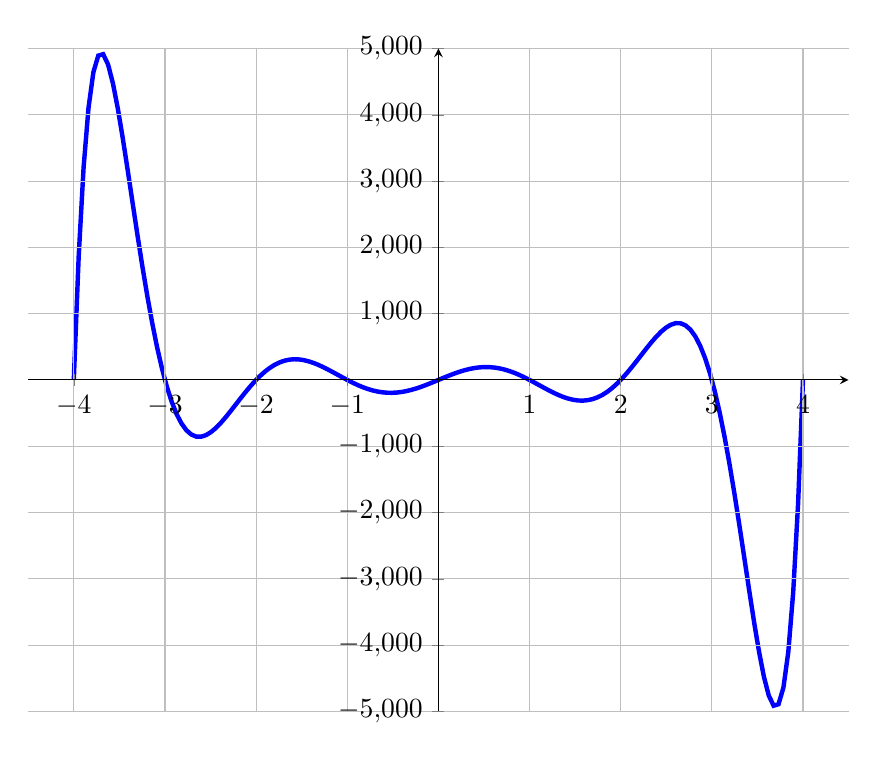
\begin{tikzpicture}
\def\FunctionF(#1){((#1)+4) * ((#1)+3) * ((#1)+2) * ((#1)+1) * ((#1)-0) * ((#1)-1) * ((#1)-2) * ((#1)-3) * ((#1)-4)}%
\begin{axis}[
        axis y line=center,
        axis x line=middle,
        axis on top=true,
        xmin=-4.5,
        xmax=4.5,
        ymin=-5000,
        ymax=5000,
        height=10.0cm,
        width=12.0cm,
        grid,
        xtick={-5,...,5},
        ytick={-6000,-5000,...,6000},
    ]
    \addplot [domain=-4:4, samples=150, mark=none, ultra thick, blue] {\FunctionF(x)};
\end{axis}
\end{tikzpicture}
\end{center}

\begin{itemize}
 \item[$\rightarrow$] 2b) Gleichverteilte Stützstellen sind böse!
 \item[$\rightarrow$] Intuitiv: wir brauchen mehr Stützstellen am Rand.
  \item[$\rightarrow$] Formal: Finde eine Stützstellenverteilung, die
  \begin{equation*}
    \max_{x\in[a,b]} \abs{ w(x) }
  \end{equation*}
  minimiert.
\end{itemize}

Um die Notation einfach zu halten, beschänken wir uns ab jetzt auf das Intervall $[-1,1]$.

\begin{definition}
 Das $n$-te Tschebyscheff-Polynom ist
 \begin{equation*}
    T_n(x) = \cos( n \arccos x ),\qquad x\in[-1,1]
 \end{equation*}
\end{definition}

Eigenschaften:
\begin{enumerate}
 \item Ja, das ist wirklich ein Polynom! (von Grad $n$)
 \item Die Koeffizienten sind ganzzahlig, der höchste ist $2^{n-1}$.
 \item $\abs{T_n(x)} \leq 1$ für $x\in[-1,1]$.
 \item Die Nullstellen sind
 \begin{equation*}
    x_k = \cos\left( \frac{2k-1}{2n} \pi\right) \quad k=1,\hdots,n\quad \text{keine doppelten!}
 \end{equation*}

\end{enumerate}


\begin{satz}
 Das Tschebyscheff-Polynom $T_n$ ist minimal bzgl.
 \begin{equation*}
    \norm{ f}_\infty = \max_{x\in [-1,1]} \abs{ f(x)}
 \end{equation*}
 unter allen Polynomen vom Grad $n$ mit führenden Koeffizienten $2^{n-1}$.

\end{satz}

Was nützt uns das?
\begin{itemize}
 \item Wir suchen Stützstellen $x_0,\hdots,x_n$ so dass
 \begin{equation*}
    \max_{x\in [-1,1]} \abs{ w(x)} = \max_{x\in [-1,1]} \abs{ (x-x_0)(x-x_1)\cdots (x-x_n)}
 \end{equation*}
 minimal wird.
 \item $w$ ist Polynom vom Grad $n+1$, und normiert.
 \item Das kleinste normierte Polynom vom Grad $n+1$ auf $[-1,1]$ ist $\frac{T_{n+1}}{2^{n}}$.
 \item[$\Rightarrow$] Wähle $x_0,\hdots,x_n$ als die Nullstellen von $T_{n+1}$.

\end{itemize}

\todoannot{\baselineskip}{Bilder der Tschebyscheff-Polynome}

\todoannot{\baselineskip}{Computer: Interpolation mit Tschebyscheff-Polynomen}



%%%%%%%%%%%%%%%%%%%%%%%%%%%%%%%%%%%%%%%%%%%%%%%%%%%%%%%%%%%%%%%%%%%%%%%%%%%%%%%%%%%%%%%%%%%%%%%%%%%%

\section{Spline-Interpolation}

 Bisher: Interpolation mit einem Polynom. Funktioniert, \emph{aber}:
\begin{itemize}
  \item Wird stark oszillatorisch, wenn die Anzahl der Stützstellen (also der Polynomgrad) groß wird.
  \item[$\Rightarrow$] Verbesserung: Nutze Nullstellen der Tschebyscheff-Polynome als Stützstellen.
\end{itemize}

\textbf{ABER}:
\begin{itemize}
  \item Häufig kann man sich die Lage der  Stützstellen nicht aussuchen.
  \item Häufig hat man \emph{sehr viele} Stützstellen!
\end{itemize}

\underline{Alternativer Ansatz:} Wir interpolieren mit stückweisen Polynomen.

\bigskip

Sei $\Delta$ eine Zerlegung von $\left[a, b\right]$ durch Stützstellen: 
\begin{equation*}
 a = x_0<x_1<\dots < x_n=b.
\end{equation*}

\begin{defi}
  Ein Spline vom Grad $m$ mit Glattheit $l\in \mathbb{N}$ zur Zerlegung $\Delta$ ist eine Funktion $s:\left[a, b\right] \rightarrow \mathbb{R}$ so dass:
  \begin{itemize}
    \item $s \in C^l([a, b])$,
    \item für alle $k=0, \dots, n-1$ ist die Einschränkung $s_k = s|_{[x_k, x_{k+1}]}$ ein Polynom vom Grad höchstens $m$.
  \end{itemize}
  Die Menge aller dieser Funktionen bezeichnen wir mit $S_m^l(\Delta)$. 
\end{defi}

\underline{Worterklärung:} Spline $\rightarrow$ englisch für \glqq Straklatte\grqq, eine Art Kurvenlineal, die im Schiffsbau verwendet wird.

\medskip

Jünger als Polynome: Die erste Erwähnung des Wortes \glqq Spline\grqq{} findet sich in 1946.\newline

Am weitaus häufigsten kommen kubische Splines (also stückweise kubische Polynome) zur Anwendung.

Warum ? 
\begin{itemize}
  \item Einerseits: einfach, Ordnung niedrig.
  \item Andererseits: Man kann damit $C^2$-Funktionen bauen.
\end{itemize}

Stetigkeit der zweiten Ableitung ist für viele Anwendungen sehr wichtig!


\subsection{$C^1$-Interpolation}

Seien $f_0, \dots, f_n$ Stützwerte an den Stützstellen $x_0, \dots, x_n$. Wir suchen eine Funktion $s \in S^1_3(\Delta)$ mit $s(x_i) = f_i$ für alle $i=0,\dots, n$.
\begin{itemize}
  \item Auf jedem Intervall: $s$ ist Polynom dritten Grades. \newline
  $\rightarrow$ 4 Parameter, aber die Interpolationsbedingungen legen nur zwei davon fest.

  \item Weiterhin fordern wir Stetigkeit der Ableitung.

   Das gibt eine weitere Bedingung pro Intervall.

  \item Eine Bedingung ist immer noch frei!

  Man kann den Wert der Ableitung an den Stützstellen vorgeben (Hermite-Interpolation).

  \item Seien $m_0, \dots, m_n$ weitere Werte an den Stützstellen.\newline
  $\rightarrow$ Die $m_i$ werden die Ableitung von $s$ an den $x_i$
\end{itemize}

Auf dem Intervall $\left[x_k, x_{k+1}\right]$ machen wir jetzt folgenden Ansatz: 
\[ s_k(x)= a_k(x-x_k)^3 + b_k(x-x_k)^2 + c_k(x-x_k) + d_k\]

\emph{Ziel:} Berechne $a_k, b_k, c_k, d_k$ aus $f_k, f_{k+1}, m_k, m_{k+1}$.
\begin{enumerate}
  \item $s_k(x_k)=d_k = f_k$
  \item $s_k'(x_k) = c_k = m_k$
\end{enumerate}

\medskip

Jetzt interessant: Wert und Ableitung an der Stelle $x_{k+1}$.

\medskip

$\rightarrow$ Setze zur Abkürzung: $h_k = x_{k+1} - x_k$.
Dann ist:
\begin{equation*}
 s_k(x_{k+1}) = a_k h_k^3 + b_k h_k^2 + m_k h_k + f_k = f_{k+1}
\end{equation*}

Da sieht man noch nichts, also noch die Ableitung
\begin{equation*}
 s'_{k}(x_{k+1}) = 3a_kh_k^2 + 2b_k h_k + m_k = m_{k+1}.
\end{equation*}

Dies ist ein lineares Gleichungssystem:

\begin{equation*}
\begin{pmatrix}
h_k^3 & h_k^2 \\
3h_k^2 & 2h_k
\end{pmatrix} 
\begin{pmatrix}
a_k \\
b_k
\end{pmatrix} = 
\begin{pmatrix}
f_{k+1} - m_kh_k - f_k\\
m_{k+1} - m_k
\end{pmatrix}.
\end{equation*}

Die Matrix ist invertierbar, denn $\det(\cdot) = 2h_k^4 - 3h_k^4 = -h_k^4 \neq 0$.

\medskip

Also existiert eine eindeutige Wahl der Parameter $a_k, b_k$.

\begin{satz}
  Sei eine Zerlegung $\Delta$ des Intervalls $\left[a, b\right]$ gegeben.
  Dann gibt es für beliebige Zahlen $f_0, \dots, f_n$ und $m_0, \dots, m_n$ genau ein Spline $s\in S^1_3(\Delta)$ mit
 \begin{equation*}
  s(x_k) = f_k \text{ und } s'(x_k) = m_k,
  \qquad
  \forall k =0, \dots, n.
 \end{equation*}
\end{satz}

\begin{itemize}
  \item Wo kommen die $m_k$ her?
  \item Möglicherweise sind die Ableitungen von $f$ bekannt (Hermite- Interpolation)! Und wenn nicht?
  \item Die Interpolierende $s$ ist $C^1$, aber nicht $C^2$.
\end{itemize}

\underline{Idee:} Wähle die $m_k$ so, dass $s$ \emph{zwei}mal stetig differenzierbar wird.

\subsection{Kubische $C^2$-Splines}

\begin{itemize}
  \item $C^2$ heißt: $s_k''(x_{k+1}) = s_{k+1}''(x_{k+1}), \; \forall k=0, \dots, n-2$
  \item Mit den vorherigen Ansatz für $s_k$:
   \begin{equation*}
    s''_k(x_{k+1}) = 6a_k(x-x_k) + 2b_k
   \end{equation*}
   also
   \begin{equation*}
    s''_k(x_{k+1}) = 6 a_kh_k + 2b_k
    \qquad
    s''_{k+1}(x_{k+1}) = 2b_{k+1}
   \end{equation*}
   \begin{equation}
    \label{eq:interpolation:cubic_spline_continuity}
    \Rightarrow 3a_kh_k + b_k = b_{k+1}
   \end{equation}

  \item Hier hängen also die Polynomkoeffizienten für die unterschiedlichen Teilintervalle
    voneinander ab.
\end{itemize}

\subsubsection{Ausrechnen der Koeffizienten $a_k, b_k$}

\begin{itemize}
  \item Bisher wissen wir nur, dass die Koeffizienten das lineare Gleichungssystem
   \begin{equation*}
    \begin{pmatrix}
   h_k^3 & h_k^2 \\
   3h_k^2 & 2h_k
   \end{pmatrix}
   \begin{pmatrix}
   a_k \\
   b_k
   \end{pmatrix}
   =
   \begin{pmatrix}
   f_{k+1} - m_kh_k - f_k\\
   m_{k+1} - m_k
   \end{pmatrix}
  \end{equation*}
 lösen.
\end{itemize}

Die Lösung davon ist:
\begin{align*}
 a_k & = - \frac{2}{h_k^3}(f_{k+1} - f_k) + \frac{1}{h_k^2}(m_k + m_{k+1}) \\
 %
 b_k & = \frac{3}{h_k^2}(f_{k+1} - f_k) - \frac{1}{h_k}(2m_k + m_{k+1}).
\end{align*}

Einsetzen in~\eqref{eq:interpolation:cubic_spline_continuity}:
\begin{multline*}
 \underbrace{-\frac{6}{h_k^2}(f_{k+1} - f_k) + \frac{3}{h_k}(m_k + m_{k+1})}_{3a_kh_k}
  + \underbrace{\frac{3}{h_k^2}(f_{k+1} - f_k) - \frac{1}{h_k}(2m_k + m_{k+1})}_{b_k}\\
 =
 \underbrace{\frac{3}{h^2_{k+1}}(f_{k+2} - f_{k+1}) - \frac{1}{h_{k+1}}(2m_{k+1} + m_{k+2})}_{b_{k+1}}
\end{multline*}

Umstellen:
\begin{equation*}
 \frac{1}{h_k}(m_k + 2m_{k+1}) + \frac{1}{h_{k+1}}(2m_{k+1} + m_{k+2})
 =
 \frac{3}{h_k^2}(f_{k+1} - f_k) + \frac{3}{h^2_{k+1}}(f_{k+2} - f_{k+1}).
\end{equation*}

Erweitern mit $h_k h_{k+1}$:
\begin{equation*}
 h_{k+1}m_k + 2(h_{k+1}+h_k)m_{k+1} + h_km_{k+2}
 =
 \frac{3h_{k+1}}{h_k}(f_{k+1} - f_k) + \frac{3h_k}{h_{k+1}}(f_{k+2} - f_{k+1})
\end{equation*}

Lineares Gleichungssystem!
\begin{itemize}
  \item $n+1$ Variablen, aber nur $n-1$ Gleichungen.
  \item Rang: $n-1$. Lösbar, aber nicht eindeutig lösbar.
\end{itemize}

Natürlich nicht: Wir haben $m_0$ und $m_n$ noch nicht festgelegt!

\bigskip

\underline{Randbedingungen:}

Verschiedene Möglichkeiten:
\begin{enumerate}
  \item Natürliche Randbedingungen
   \begin{equation*}
    s''(x_0) = s''(x_n) = 0.
   \end{equation*}

  \item Vollständige Randbedingungen
   \begin{equation*}
    s'(x_0) = f'(a), \;\; s'(x_n) = f'(b).
   \end{equation*}

  \item Periodische Randbedingungen
   \begin{equation*}
    s'(x_0) = s'(x_n), \;\; s''(x_n) = s''(x_n).
   \end{equation*}
  \item etc...
\end{enumerate}

\bigskip

Das Gleichungssystem ist \emph{tridiagonal}!  Damit ist es in $O(n)$ Schritten lösbar
(Thomas-Algorithmus)!


\subsection{Interpolationsfehler}

Es existieren viele Abschätzungen für den Fehler in diversen Normen, auch Fehler der Ableitung.

\bigskip

Eine der besten:

\begin{satz}[{\citet{hall_meyer:1976}}]
 Sei $\Delta$ eine Zerlegung, und setze $h \colonequals \max\vert x_{k+1} - x_k\vert$.
 Sei $f\in C^4(\left[a, b\right])$ und sei $s \in S^2_3(\Delta)$ die Spline-Interpolierende mit natürlichen
 Randbedingungen (d.h., $s''(a) = s''(b) = 0$. Dann gilt
 \[
  \norm{f - s}_\infty \leq \frac{5}{384}h^4 \norm{f^{(4)}}_\infty.
 \]
\end{satz}

Beachte: Resultat ist unabhängig von der Lage der Stützstellen!
\begin{itemize}
  \item Beweis leider zu lang zum Vorrechnen.
\end{itemize}
Hier ein schwächeres Resultat als Alternative:

\medskip

Definiere dafür die $2$-Norm
\begin{equation*}
 \norm{f}_2 \colonequals \sqrt{\int_a^b\vert f(x)\vert^2\,dx}.
\end{equation*}

\begin{satz}
  Sei $\Delta$ eine Zerlegung von $\left[a, b\right]$ und $f \in C^2(\left[a, b\right])$.
  Sei $s\in S_3^2(\Delta)$ die Spline-Interpolierende mit natürlichen oder vollständigen Randbedingungen.
  Dann ist
  \begin{equation*}
   \norm{f-s}_\infty \leq \frac{1}{2}h^{\frac{3}{2}}\norm{f''}_2.
  \end{equation*}
\end{satz}

\begin{proof}
\begin{itemize}
 \item Setze $r = f-s$.

 \item $r$ hat mindestens die $n+1$ Nullstellen $x_0, \dots, x_n$.

 \item Satz von Rolle: $r'$ hat mindestens $n$ Nullstellen.

 \item Zwei benachbarte Nullstellen von $r'$ sind höchstens $2h$ voneinander entfernt.

 \item $r'$ ist stetig, $[a, b]$ kompakt
     $\Rightarrow \exists z \in [a, b]$ mit $\abs{r'(z)} = \norm{r'}_\infty$.

 \item Sei $z_0$ die $z$ am nächsten gelegene Nullstelle von $r'$:\\
    $\Rightarrow \abs{z - z_0} \leq \frac{1}{2} \cdot 2 h = h$.

 \item Sei O.B.d.A.\ $z_0 \leq z$.

 \item Rechnen:
  \begin{align*}
   \norm{r'}^2_\infty
   & =
   \abs{r'(z)}^2 = \abs{r'(z) \underbrace{- r'(z_0)}_{0}}^2 \\
   & =
   \Big\lvert\int_{z_0}^z r''(x)\,dx \Big\rvert^2.
  \end{align*}
  \medskip
Cauchy-Schwarz: $\vert \langle x, y\rangle\vert^2 \leq \langle x,x\rangle\langle y,y\rangle$
  \begin{align}
   \nonumber
   & =
   \Big\lvert\int_{z_0}^z r''(x) \cdot 1 \,dx \Big\rvert^2
   \leq
   \int_{z_0}^z (r''(x))^2\,dx \cdot \int_{z_0}^z 1\,dx \\
   \label{eq:interpolation:bound_on_r_prime}
   & \leq
   h \norm{r''}_2^2.
  \end{align}
\end{itemize}

Jetzt der gleiche Trick für $r$ selbst:

\begin{itemize}
 \item $\exists y \in [a,b]$ so dass $\abs{r(y)} = \norm{r}_\infty$.

 \item Sei $y_0$ die $y$ am nächsten liegende Nullstelle von $r$.

 \item O.B.d.A.\ $y_0\leq y$.

 \item Rechnen:
  \begin{align*}
    \norm{r}_\infty
    & =
    \abs{r(y) - r(y_0)}
    =
    \Big\vert \int_{y_0}^y r'(x)\,dx \Big\vert \\
    & \leq
    \norm{r'}_\infty\int_{y_0}^y dx
    =
    \frac{h}{2}\norm{r'}_\infty.
  \end{align*}

 \item Einsetzen von~\eqref{eq:interpolation:bound_on_r_prime}:
  \begin{equation*}
   \norm{r}_\infty \leq \frac{h}{2}\sqrt{h}\norm{r''}_2.
  \end{equation*}

 \item Also
   \begin{equation*}
    \norm{f-s}_\infty\leq \frac{1}{2}h^{\frac{3}{2}}\norm{f'' - s''}_2.
    \qedhere
   \end{equation*}

\end{itemize}

\end{proof}

\textbf{Verwunderung:} Rechts soll $\norm{f''}_2$ stehen, nicht $\norm{f'' - s''}_2$?!?

\medskip

Das gilt auch, denn es ist immer $\norm{f'' - s''}_2 \leq \norm{f}_2$!

\bigskip

Wie beweist man das?

\medskip

Dreiecksungleichung? Nein, denn
\begin{equation*}
 \norm{f''}
 =
 \norm{f'' - s'' + s''}
 \leq
 \norm{f'' - s''} + \norm{s''}
\end{equation*}

Erstaunlich: es gilt die Dreiecks-Ungleichung mit Gleichheit!
\begin{satz}
\label{thm:interpolation:pythagoras}
 Es gilt
 \begin{equation*}
  \norm{f''}_2^2 = \norm{f'' - s''}_2^2 + \norm{s''}^2_2,
 \end{equation*}
 also insbesondere
 \begin{equation*}
  \norm{f'' - s''} \leq \norm{f''}.
 \end{equation*}
\end{satz}

\emph{Beachte:} Mit dem Satz des Pythagoras kann man das wie folgt interpretieren:\\

\medskip

   $f''- s''$ steht senkrecht auf $s''$ im Sinne des Skalarprodukts $\langle v,w\rangle = \int_{a}^bvw\,dx$.

\begin{proof}
Wir zeigen $\norm{f''}^2_2 - \norm{f'' - s''}_2^2 = \norm{s''}_2^2$.

\bigskip
Rechnen:
\begin{align*}
 \norm{f''}_2^2 - \norm{f'' - s''}_2^2
 &=
 \int_{a}^b(f''(x))^2\,dx - \int_{a}^b(f''(x) - s''(x))^2\,dx\\
 &=
 \int_{a}^b \bigg[ \underbrace{(f''(x))^2 - (f''(x))^2}_{= 0} + 2f''(x)s''(x) - (s''(x))^2 \underbrace{- (s''(x))^2 + (s''(x))^2}_{=0} \bigg] \,dx\\
 &=
 2\underbrace{\int_{a}^b(f''(x) - s''(x))s''(x)\,dx}_{\equalscolon J}
   + \underbrace{\int_{a}^b(s''(x))^2\,dx}_{= \norm{s''(x)}_2^2}.
\end{align*}

Wir zeigen $J=0$ (Beachte: $J$ ist das $L_2$-Skalarprodukt von $f''-s''$ und $s''$, und $J=0$
bedeutet gerade dass diese zwei Vektoren senkrecht aufeinander stehen!)

\bigskip

Partielle Integration:
\begin{equation*}
 J = \underbrace{(f'-s')s''\Big|_a^b}_{J_1} - \underbrace{\int_a^b (f'-s')s'''\,dx}_{J_2}
\end{equation*}

\begin{enumerate}
 \item $J_2 = 0$, denn $s'''$ ist auf jedem Teilintervall konstant, und damit
 \begin{align*}
  J_2
  & =
  \sum_{k=0}^{n-1}s'''\left(\frac{x_k+x_{k+1}}{2}\right)\int_{x_k}^{x_{k+1}}(f'-s')\,dx\\
  &=
  \sum_{k=0}^{n-1}s'''\left(\frac{x_k+x_{k+1}}{2}\right)\big(f - s\big)\Big|_{x_k}^{x_{k+1}}\\
  &=
  0.
 \end{align*}

 \item Weiterhin soll $J_1 = (f'(b)-s'(b))s''(b) - (f'(a)-s'(a))s''(a)$ gleich 0 sein.

 Dies gilt wenn man die Randbedingungen passend wählt, z.B.:
  \begin{itemize}
     \item Natürliche Randbedingungen: $s''(a) = s''(b) = 0$
     \item Vollständige Randbedingungen: $f'(a) - s'(a)=0$, $f'(b) - s'(b) =0$
     \qedhere
  \end{itemize}
\end{enumerate}
\end{proof}

Aus
\begin{equation*}
 \norm{f''}_2^2 - \norm{f'' - s''}_2^2
 =
 \norm{s''}_2^2
\end{equation*}
folgt
\begin{equation*}
 \norm{s''}_2
 \leq
 \norm{f''}_2.
\end{equation*}

\begin{kor}
 $s$ minimiert $\norm{\cdot\,''}_2$ in der Menge aller $C^2$-Funktionen die die Interpolations- und Randbedingungen erfüllen.
\end{kor}
\begin{proof}
\begin{itemize}
 \item Sei $\tilde{s}$ eine $C^2$-Funktion die die Rand- und Interpolationsbedingungen erfüllt,
   und $\norm{\tilde{s}''}_s < \norm{s''}_2$.

 \item Dann ist $s$ auch Spline-Interpolierende von $\tilde{s}$.

 \item Mit Satz~\ref{thm:interpolation:pythagoras}: $\norm{s''}_2 \le \norm{\tilde{s}''}_s$.

 \item Widerspruch!
\end{itemize}

\end{proof}



\subsection{Geometrische Interpretation}

Konstrukteure wollen Kurven, die so glatt wie möglich sind.

\bigskip

Was heißt hier \glqq so glatt wie möglich\grqq{}?
\begin{itemize}
 \item  \glqq So gerade wie möglich, keine unnötige Kurve\grqq

 \item Die \glqq Krümmung\grqq{} soll möglichst gering sein.
\end{itemize}

\bigskip

Was ist die Krümmung einer ebenen Kurve ?
\begin{itemize}
  \item Gerade: Krümmung $=0$.
  \item Kreis: Krümmung konstant $= \frac{1}{r}$
  \item Allgemeine Kurve: Inverser Radius des Schmiegekreises.
    (Der Kreis, der eine Kurve an einem Punkt am besten annähert.)

\begin{center}
\begin{tikzpicture}[scale =2]
  \draw (0,0.5) circle (0.5);
  \draw[domain=-1:1.5,samples=100,color=black] plot ({\x},{\x*\x)});
  \draw[<->] (0,0) to[out=90,in=-90]  (0,0.5);
  \node (draw) at (-0.1,0.25) {$r$};
\end{tikzpicture}
\end{center}

\end{itemize}
Sei die Kurve Graph einer Funktion $g:\mathbb{R}\rightarrow\mathbb{R}$.

\begin{itemize}
  \item Krümmung von $g$ ist $\frac{g''(x)}{\left(1+(g'(x))^2\right)^{\frac{3}{2}}}$.
  \item Falls $g'$ klein ist ist das $\approx g''$
\end{itemize}

$\Rightarrow$\glqq Kubische Splines minimieren die Krümmung\grqq.

\subsection{B-Splines}

\begin{itemize}
 \item Basis-Splines

 \item Entwickelt in den 1950ern und 1960ern in der Luftfahrt- und Automobilindustrie.
\end{itemize}

\textbf{Keine} neue Art von Funktionen!

\medskip

Sstattdessen: Einen neue Basis für den Spline-Raum $S_m^l(\Delta)$.

\begin{itemize}
  \item Problem mit der alten Basis: Basis ist global: jeder Wert $f_k$, $k=0, n$ beeinflusst den Wert der Splinefunktion auf ganz $\left[a,b\right]$.
  \item Kein Problem, wenn die Stürtzwerte $f_i$ fest gegeben sind.

  \item Aber: Problem, wenn Splines zum Modellieren von Kurven und Flächen verwendet werden.

  \item Deshalb: konstruiere lokale Basis von $S_m^l(\Delta)$

    (D.h.\ Basisfunktionen haben lokalen Träger)

  \item Beschreibe Funktionen/ Kurven/ Flächen durch Koeffizienten bzgl dieser Basis!
    Solche Splines sind nicht interpolierend. In der Modellierung ist das aber egal.
\end{itemize}

\begin{defi}
 Sei $x_1\leq \dots \leq x_n$ eine Folge von Knoten (d.h.: Stützstellen).
 Dann sind die B-Splines $N_p(x)$ der Ordnung $p$ für $p=1, \dots, n$ und $i=1, \dots, n-p$ erklärt durch:
 \begin{equation*}
  N_{k,1}(x)
  \colonequals
  \begin{cases}
   1 & \text{falls $x_k\leq x <x_{k+1}$},\\
   0 & \text{sonst.}\\
  \end{cases}
 \end{equation*}
 \begin{equation*}
  N_{k,p}(x)
   \colonequals
  \frac{x - x_k}{x_{k+p-1} - x_k}N_{k,p-1}(x) + \frac{x_{k+p} - x}{x_{k+p} - x_{k+1}}N_{k+1, p-1}(x)
 \end{equation*}
\end{defi}

\begin{bsp}
  \begin{itemize}
    \item $p=1$: \[N_{k,1}(x) := \left\{\begin{array}{ccc}
1& \;\text{falls}\; x_k\leq x <x_{k+1}\\
0& \,\text{sonst.}\\
\end{array}\right.\]

  \begin{center}
\begin{tikzpicture}[scale =2]
  \draw (-2,0) node[above]{$x_{k-1}$};
  \fill (-2,0) circle(0.4mm);
  \draw (-1,0) node[above]{$x_{k}$};
  \fill (-1,0) circle(0.4mm);
  \draw (0,0) node[above]{$x_{k+1}$};
  \fill (0,0) circle(0.4mm);
  \draw (1,0) node[above]{$x_{k+2}$};
  \fill (1,0) circle(0.4mm);
  \draw[->] (-3,0) -- (3,0);
  \draw (-1,1) -- (0,1);
  \draw[dashed] (-1,1) -- (-1,0);
  \draw[dashed] (0,1) -- (0,0);
\end{tikzpicture}
\end{center}

  \item $p=2$:
\begin{align*}
 N_{k,2}(x) &= \frac{x - x_k}{x_{k+1} - x_k}\chi _{\left[x_k, x_{k+1}\right]}(x) + \frac{x_{k+2} - x}{x_{k+2} - x_{k+1}}\chi _{\left[x_{k+1}, x_{k+2}\right]}(x)\\
&= \left\{\begin{array}{ccc}
\frac{x - x_k}{x_{k+1} - x_k}& \;\text{falls}\; x_k\leq x \leq x_{k+1}\\
\frac{x_{k+2} - x}{x_{k+2} - x_{k+1}}& \;\text{falls}\; x_{k+1}\leq x \leq x_{k+2}\\
0& \,\text{sonst.}\\
\end{array}\right.
\end{align*}

\begin{center}
\begin{tikzpicture}[scale =2]
  \draw (-2,0) node[above]{$x_{k-1}$};
  \fill (-2,0) circle(0.4mm);
  \draw (-1,0) node[above]{$x_{k}$};
  \fill (-1,0) circle(0.4mm);
  \draw (0,0) node[above]{$x_{k+1}$};
  \fill (0,0) circle(0.4mm);
  \draw (1,0) node[above]{$x_{k+2}$};
  \fill (1,0) circle(0.4mm);
  \draw[->] (-3,0) -- (3,0);
  \draw (-1,0) -- (0,1);
  \draw (0,1) -- (1,0);
\end{tikzpicture}
\end{center}
\begin{itemize}
  \item $p\rightarrow p+1$ Stückweise Multiplikation mit Linearfaktor

    $\Rightarrow$ $N_{k,p}$ ist stückweises Polynom der Ordnung $p-1$.

  \item Information aus $p$ Intervallen $\Rightarrow$ lokaler Träger
  \end{itemize}
\item $p=3$
\begin{center}
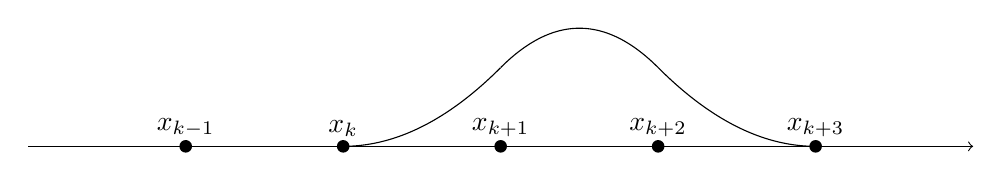
\begin{tikzpicture}[scale =2]
  \draw (-2,0) node[above]{$x_{k-1}$};
  \fill (-2,0) circle(0.4mm);
  \draw (-1,0) node[above]{$x_{k}$};
  \fill (-1,0) circle(0.4mm);
  \draw (0,0) node[above]{$x_{k+1}$};
  \fill (0,0) circle(0.4mm);
  \draw (1,0) node[above]{$x_{k+2}$};
  \fill (1,0) circle(0.4mm);
  \draw (2,0) node[above]{$x_{k+3}$};
  \fill (2,0) circle(0.4mm);
  \draw[->] (-3,0) -- (3,0);
  \draw[domain=-1:0,samples=100,color=black] plot ({\x},{(\x+1)^2/2});
  \draw[domain=0:1,samples=100,color=black] plot ({\x},{(-2*(\x+1)^2+6*(\x+1)-3)/2});
  \draw[domain=1:2,samples=100,color=black] plot ({\x},{(2-\x)^2/2});
\end{tikzpicture}
\end{center}
\end{itemize}
\end{bsp}

\underline{Eigenschaft:} 
\[N_{k,p}(x)\geq 0, \qquad \forall k, p, x\]

Darstellung von Spline-Funktionen:
\[s(x) = \sum_{k=1}^n f_kN_{k,p}(x)\]

Achtung: es gilt NICHT $s(x_k) = f_k$ !

\underline{Ableitung:} 

\[ N'_{k, p}(x)= (p-1)\left(\frac{-N_{k+1, p-1}(x)}{x_{k+p} - x_{k+1}}+\frac{N_{k, p-1}(x)}{x_{k+p-1}-x_k}\right)\]


Großer Vorteil: Man kann die Glattheit der Funktionen an den Stützstellen kontrollieren, indem man mehrfache Stützstellen zulässt.

\begin{satz}
  Sei $x$ ein $m$-facher Knoten, d.h
\[x_{j-1} < x_j = x_{j+1} \dots = x_{j+m-1} < x_{j+m}\]
Dann ist $N_{k,p}$ an der Stelle $x_j$ mindestens $p-1-m$-mal stetig differenzierbar.
\end{satz}
